\taskpic{ Стеклянный шар объемом $V$ и плотностью $\rho$ находится в
  сосуде с водой. Угол между стенкой сосуда и горизонтальным дном
  $\alpha$, внутренняя поверхность сосуда гладкая, плотность воды
  $\rho_0$. Найдите силу давления шара на дно сосуда, если сосуд
  движется с постоянным горизонтальным ускорением $a$. }
{
  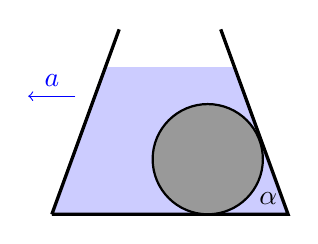
\begin{tikzpicture}
    \draw[white,fill=blue!20] (0,0) ++ (70:2cm) -- (0,0) -- (3,0)
    -- ++(110:2cm) -- cycle;
    \draw[very thick] (0,0) -- ++(70:2.5cm) (0,0) -- (3,0) -- ++
    (110:2.5cm);
    \draw[thick,fill=gray!80] (1.98,0.7) circle (0.7cm);
    \draw (2.75,0.2) node {$\alpha$};
    \draw[blue,->] (0.3,1.5) -- (-0.3,1.5) node[midway,above] {$a$};
  \end{tikzpicture}
}
% Квант, 2006, №1